%%%%%%%%%%%%%%%%%%%%%%%%%%%%%%%%%%%%%%%%%

\documentclass{academia}

\geometry{left=4.5cm,top=3cm,right=4.5cm,bottom=3cm,nohead,nofoot}

\def\firstname{Benjamin}
\def\familyname{Vial}
\def\FileSubject{cover letter}
\def\FileAuthor{\firstname~\familyname}
\def\FileTitle{\firstname~\familyname's~\FileSubject}
\def\FileKeyWords{\firstname~\familyname, \FileSubject}

  \RequirePackage[unicode]{hyperref}% unicode is required for unicode pdf metadata
  \hypersetup{
    breaklinks,
    baseurl       = http://,
    pdfborder     = 0 0 0,
    pdfpagemode   = UseNone,% do not show thumbnails or bookmarks on opening
    pdfstartpage  = 1,
%    pdfproducer   = {\LaTeX{}},% will/should be set automatically to the correct TeX engine used
    bookmarksopen = true,
    bookmarksdepth= 2,% to show sections and subsections
    pdfauthor   = {\FileAuthor},%
    pdftitle    = {\FileTitle},%
    pdfsubject  = {\FileSubject},%
    pdfkeywords = {\FileKeyWords},%
    pdfcreator  = {\LaTeX},%
    pdfproducer = {\LaTeX}
    }


\begin{document}
\hfill%
\begin{minipage}[t]{.5\textwidth}
\raggedleft{\bfseries Benjamin Vial}\\
146 Glyn Road\\
London E5 0JE, UK\\
~+44~7840~029~744\\
~\href{mailto:b.vial@qmul.ac.uk}{b.vial@qmul.ac.uk}\\
~\href{www.bvial.info}{bvial.info}
\\[2em]
\today
\end{minipage}\\[1em]
\begin{minipage}[t]{.5\textwidth}
    \begin{flushleft}
        \textbf{Queen Mary University of London}\\
Personnel dept.\\
South Kensington Campus\\
London SW7 2AZ, UK\\
    \end{flushleft}
\end{minipage}
\hfill % US style
\\[2em]
%\raggedright


Dear Professor Craster,\\[1em]


\textbf{Application to the post of Research Associate in Metamaterial Physics, Computation and Homogenisation}\\[1.em]


I am pleased to attach my CV for the post of
Research Associate in Metamaterial Physics, Computation and Homogenisation 
as advertised on the imperial.ac.uk website.

For the past seven years I have held the post of Postdoctoral Research
Assistant in the Antennas and Electromagnetics reseach group in
the School of Electronics Engineering and Computer Science
at Queen Mary University of London, where my research
has focused primarily on Applied Electromagnetism and Microwave Engineering.

I have a particular interest in Wave Physics and metamaterials, with an emphasis on numerical
modelling and inverse design tools. As detailed in my CV, I have 
broad and strong background in computational Electromagnetism 
with a emphasis on developing open-source numerical models 
to support my research (mostly in Python using the FeniCS finite element library), 
but also with commercial tools. Although my research has focused on Electromagnetism, 
I initially obtained a Masters degree in acoustics and have a stong 
knowledge of wave propagation through structured media. 


I have published widely in the field of Optics, Photonics
and Electromagnetism.
My PhD thesis, “Study of open electromagnetic resonators by modal appoach. 
Application to to infrared multispectral filtering” won two national awards in 2014, and
our recent paper "High frequency meta-ferroelectrics by inverse design", where we applied 
homogenization methods to optimize a metamaterial unit cell, was selected
in the \textit{\href{https://www.osapublishing.org/spotlight/summary.cfm?id=450295}{Spotlight on Optics}}
from the Otical society of America.


During my postdoctoral experience in QMUL, I had the
opportunity to hekp working on numerous grant applications, which led to succesful funding by the EPSRC of several major projects
for a total of around £2.3M and fruitful collaborations with research institutions
and industries accross the UK.

I am currently working on the \textit{\href{https://animate-research.com/}{ANIMATE project}},
a collaboration with the School of Engineering and Material science in QMUL,
where my research focuses on developing innovative metamaterials and
numerical models for tunable electromagnetic devices.
The cross-disciplinary approach adopted is very stimulating and aims to
pursue an end-to-end research, from modelling and material processing to
functional devices. 


In summary, I believe my relevant expertise in wave physics, mathematical modelling and 
computational methods, together with my strong research and publications record, make me ideally placed to contribute in this 
Research Assistant position.

I look forward to the opportunity to discuss my application further at
interview. Please contact me if you would like any further information
in the meantime.



Yours sincerely,\\[1.5em]


\textbf{Benjamin Vial}

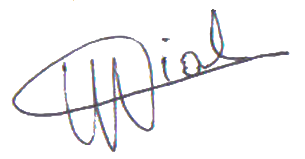
\includegraphics[width=3cm]{sig.png}
%

\end{document}
